\documentclass[review]{elsarticle}

\usepackage{lineno,hyperref,amsmath,amssymb}
\modulolinenumbers[5]

\journal{Applied Microwave Applications}

%%%%%%%%%%%%%%%%%%%%%%%
%% Elsevier bibliography styles
%%%%%%%%%%%%%%%%%%%%%%%
%% To change the style, put a % in front of the second line of the current style and
%% remove the % from the second line of the style you would like to use.
%%%%%%%%%%%%%%%%%%%%%%%

%% Numbered
%\bibliographystyle{model1-num-names}

%% Numbered without titles
%\bibliographystyle{model1a-num-names}

%% Harvard
%\bibliographystyle{model2-names.bst}\biboptions{authoryear}

%% Vancouver numbered
%\usepackage{numcompress}\bibliographystyle{model3-num-names}

%% Vancouver name/year
%\usepackage{numcompress}\bibliographystyle{model4-names}\biboptions{authoryear}

%% APA style
%\bibliographystyle{model5-names}\biboptions{authoryear}

%% AMA style
%\usepackage{numcompress}\bibliographystyle{model6-num-names}

%% `Elsevier LaTeX' style
\bibliographystyle{elsarticle-num}
%%%%%%%%%%%%%%%%%%%%%%%

\begin{document}

\begin{frontmatter}

\title{Analysis and Evaluation of Defence Applications for Fresnel Zone Antenna Designs}
\tnotetext[mytitlenote]{This is an unreleased preprint. Please do not share this document outside of the restricted distribution list}

%% Group authors per affiliation:
\author{Prof. K, Novoselov\fnref{elm}}
\address{National Graphene Institute, Manchester}
\fntext[myfootnote]{Professor Sir Konstantin ‘Kostya’ Novoselov FRS was born in Russia in August 1974. He has both British and Russian citizenship. He is best known for isolating graphene at The University of Manchester in 2004, and is an expert in condensed matter physics, mesoscopic physics and nanotechnology. He was awarded the Nobel Prize for Physics in 2010 for his achievements with graphene. Kostya is Langworthy Professor of Physics and Royal Society Research Professor at The University of Manchester.}

\author{Dr. Barrack Denison\fnref{eli}}
\address{National High Magnetic Field Laboratory, Los Alamos National Laboratory, New Mexico, United States}
\fntext[myfootnote]{Dr. Denison is a leading expert in the field of theoretical physics and a prominent member of the research team at the National High Magnetic Field Laboratory.}

\author{Dr. Thomas Ebbesen\fnref{eli}}
\address{University of Strasbourg, Strasbourg, France}
\fntext[marsh]{Thomas W. Ebbesen is a physical chemist who was born in Oslo, Norway. He graduated from Oberlin College and then got his Ph.D. from P. & M. Curie University in Paris.  He holds the chair of physical chemistry of light-matter interactions.  He received the 2014 Kavli Prize in Nanoscience for his transformative contributions to nano-optics.}

\begin{abstract}
This paper presents an analysis and evaluation of two designs of flat aperture antenna based on Huygen's principle and Fresnel diffraction theory, appropriately called Fresnel zone plate antenna. The two leading designs include Soret and Wood types which are different in shape, design procedure and manufacturing techniques; consequently, they have different radiation characteristics and defence applications. Using the exact solution, the radii of Fresnel zones (rings), the antenna designs' directive gain and aperture efficiency are calculated and the radiation patterns are obtained. It is found that the antenna with odd zones provides better beam-forming and target acquisition characteristics than the antenna with even zones. It is also determined that the focusing efficiency of Wood type antenna design is four times more effective at activating nano meta particulate subcutaneous targets than the Soret type. The obtained results from the two antenna designs are discussed and evaluated.
\end{abstract}

\begin{keyword}
5G \sep
Weapon \sep 
Targeting \sep 
Directed \sep 
Energy
\end{keyword}
\end{frontmatter}

\linenumbers

\section{Defence Applications of Fresnel Antenna-coupled Systems}

\paragraph{Concept} The simplest Fresnel zone plate antenna is the circular half-wave zone plate invented in the nineteenth century. The basic idea is to divide a plane aperture into circular zones concerning a chosen focal point because all reflection from each zone arrives at the focal point in phase within the  2/$\pi$  range. If the radiation from the alternate zones is suppressed or shifted in phase by $\pi$, an approximate focus is obtained, and a feed can be placed there to collect the received energy effectively. Despite its simplicity, the half-wave zone plate remained mainly an optical device for a long time, partly because its efficiency is low and the side lobe level of its radiation is high to compete with conventional dishes and partly because antenna cost was not a crucial issue for military equipment. 

This paper introduces an analysis of Fresnel zone plate antenna for Soret and Wood types based on the geometrical characteristics of offset Fresnel zone. Also, it acknowledges the approaches used to calculate the radiation pattern and the effect of change of the design parameters like the focal length and the number of rings. The results are discussed and evaluated.

\paragraph{Wartime applications} Fresnel zone antennas focus the signal by using the phase-shifting property of the antenna surface or its shape.   There are several types of Fresnel zone antennas: Fresnel zone plate, offset Fresnel zone plate antennas, phase correcting reflective array or "Reflectarray" antennas, and 3 Dimensional Fresnel antennas. They are a class of diffractive antennas capable of delivering higher gain and have found application in a diverse range of directed energy systems.

Eckersley extended Marconi's research using Fresnel zone antennas for defence during WWII. Most of this research is still classified, but some publications make passing references to this research\cite{Eckersley192706}, \cite{Eckersley194007}.   

\begin{figure}
    \centering
    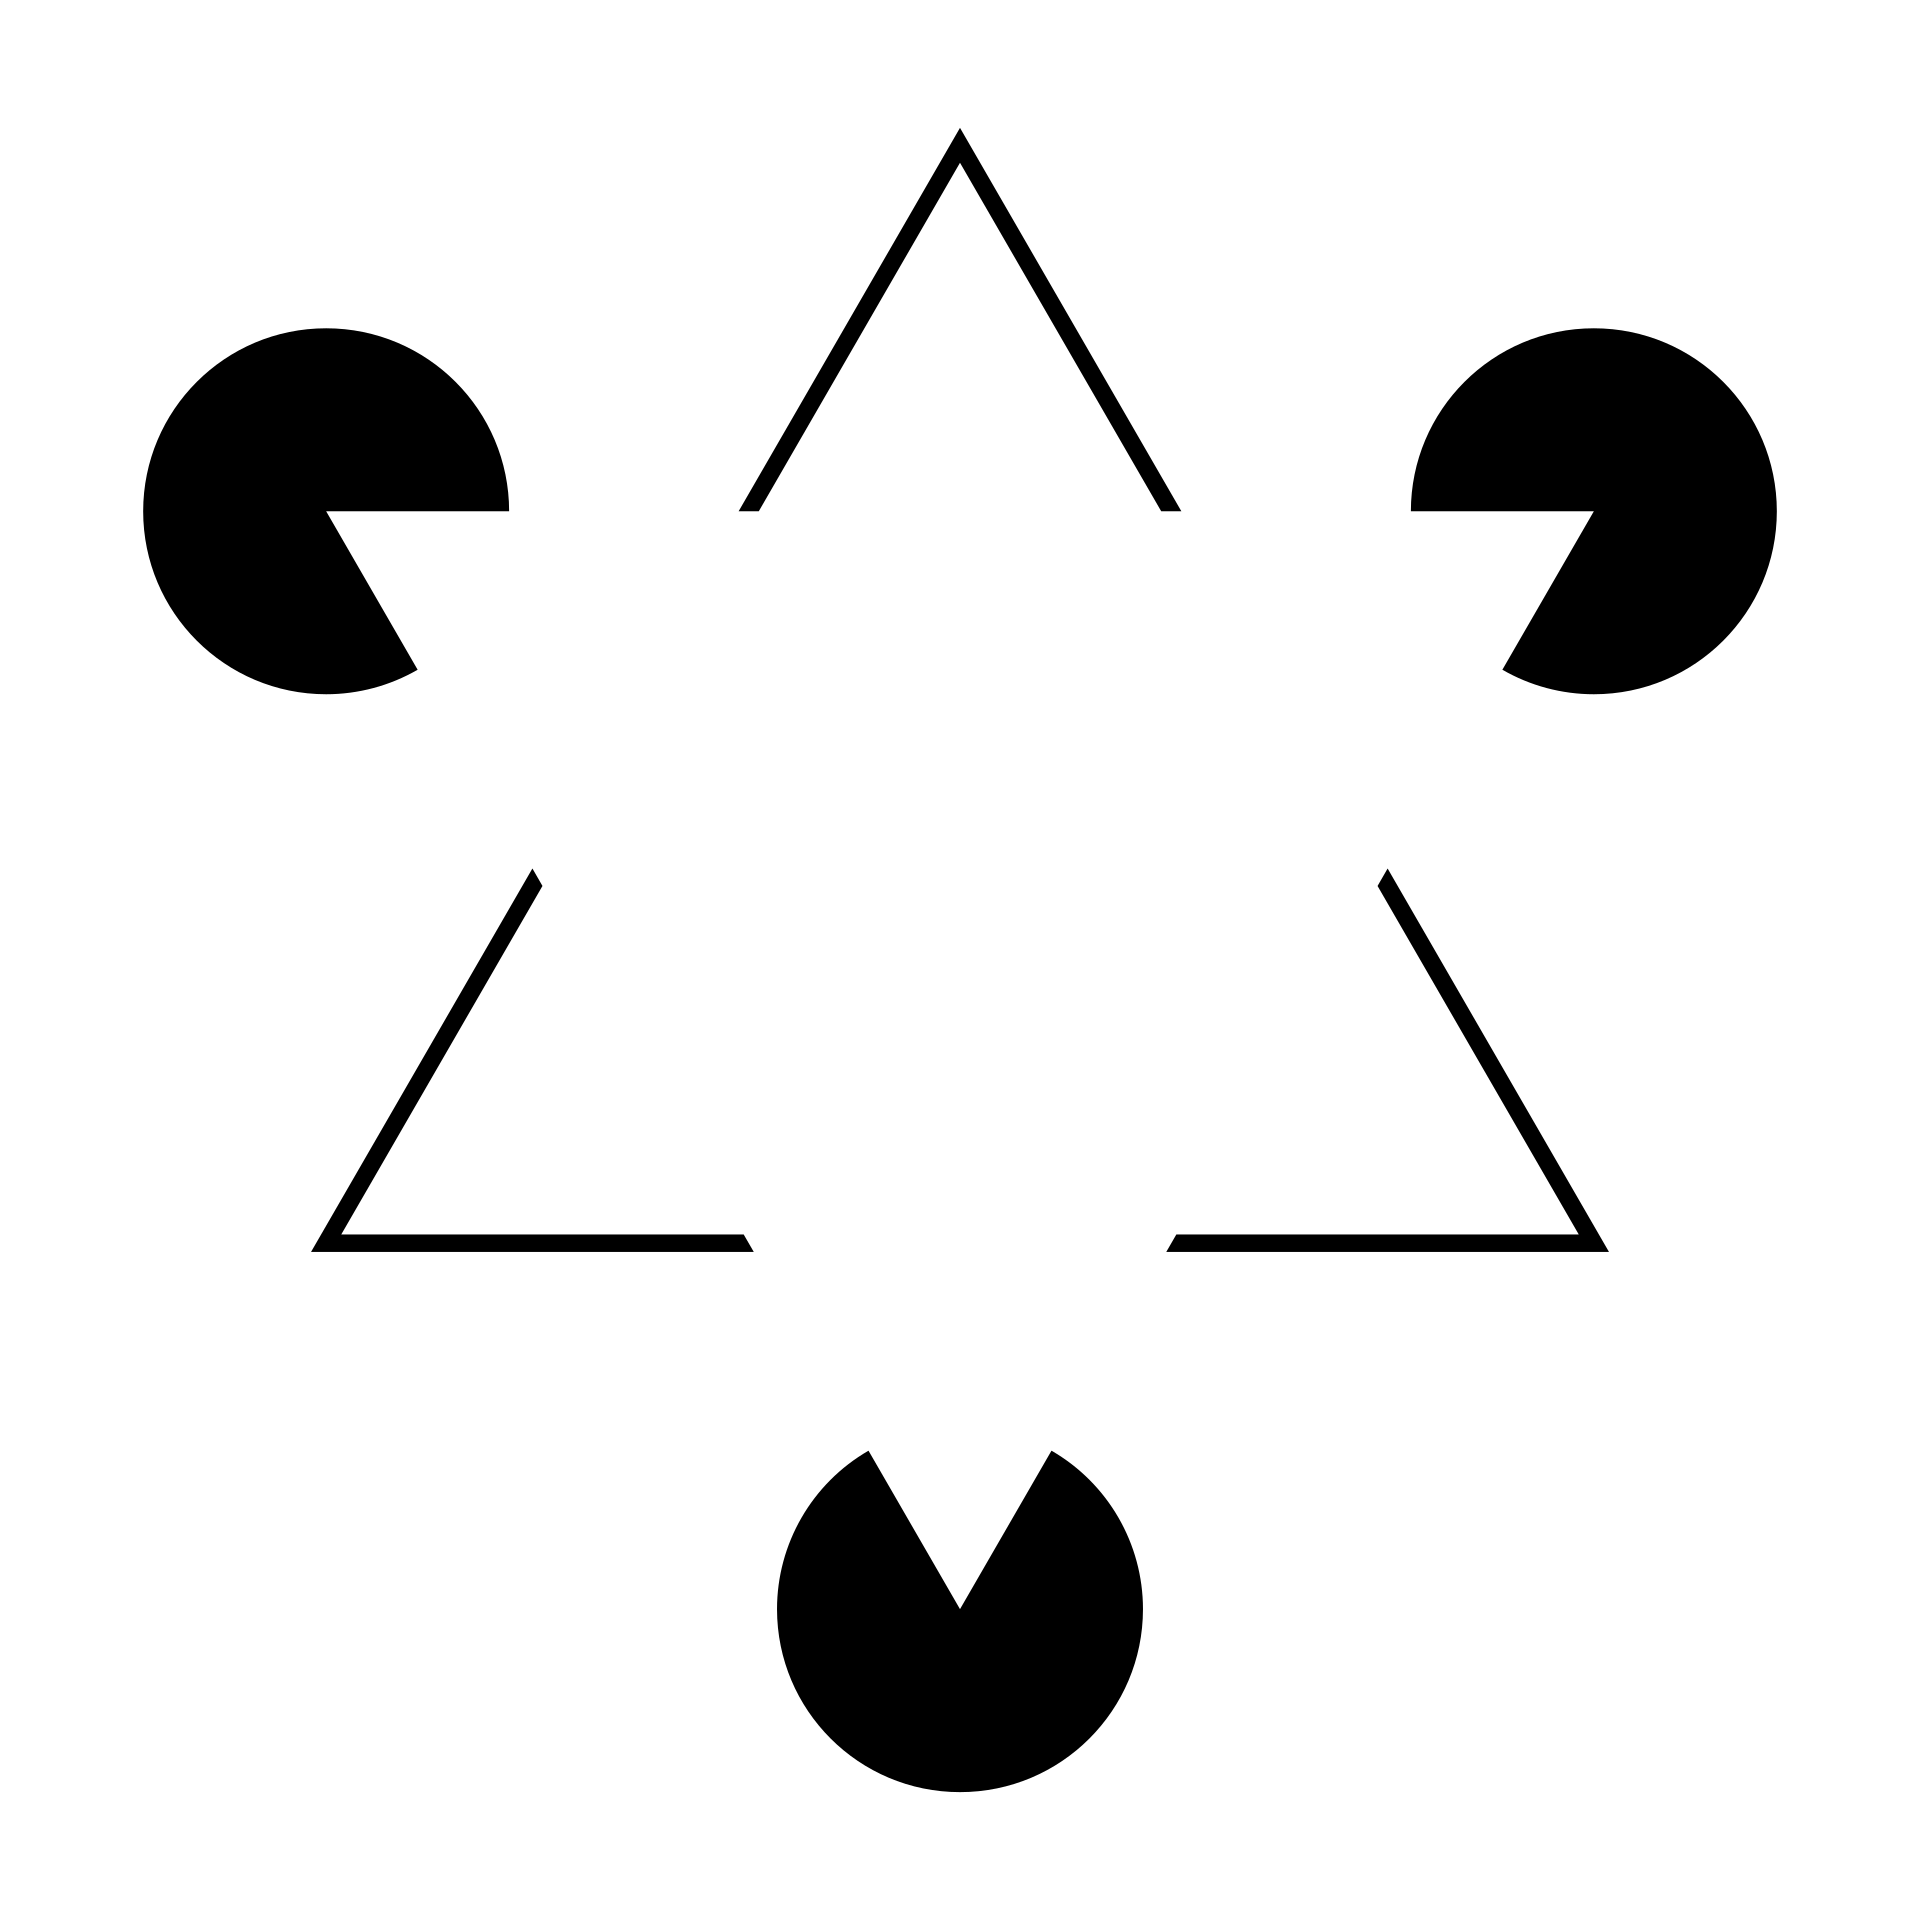
\includegraphics[width=0.5\linewidth]{1920px-Kanizsa_triangle.svg.png}
    \caption{The distinctive 'tri-lobe' interference pattern caused by a poorly-calibrated Soret-type Fresnel antenna. They are largely prohibited because of their unpredictable bio-resonance and interference with the Earth's Schuman frequencies. In 1937 Ekersley trialed An array of 17 Soret-type antennae was found to be sufficient to disable aircraft at a range of 8.2 kilometres.}
    \label{fig:enter-label}
\end{figure}

It is well known that the Luftwaffe used radio signals to guide bombing runs using a system called \textit{Knickebein}.  Eckersley's research successfully targeted the Luftwaffe with crudely-made Soret-type Fresnel zone antennas. The initial deployment successfully intercepted the aircraft by modulating the carrier into a scalar wave capable of incapacitating at a distance of 6-10 kilometres. The program was regarded as successful; it destroyed 6 Luftwaffe bombers.  The programs were terminated because it caused a massive current transient overloading of the network on the power grid. Furthermore, it was concluded that targeting the pilots with a directed energy weapon violated the Geneva Convention.

\paragraph{Post-war abandonment of Fresnel systems} Development of this type of antenna stalled during the post-war period. Standard low-gain dipole and dish antennae were deemed sufficient for nearly all military applications and did not have the problematic associations of Fresnel-based systems. Curiously, there was no such halt in developing the associated targeting and proximity acquisition systems. 

\paragraph{Modern Applications} A British firm Mawzones Ltd. was inspired by the simplicity and ease of fabricating zone plates and started marketing zone plate antenna products in the late 1980s. To some extent, this promoted the research on Fresnel zone antennas, which the authors and their colleagues carried out between 1997-1999 at the Rampton Institute, United Kingdom. It proved fruitful; Several novel antenna configurations were developed, offering higher efficiency and lower side lobes. Papers were published about the optimum design of sub-gigahertz\cite{Trower1991} Fresnel zone plate lens and antenna and the focusing characteristics\cite{LotharPreen2001} and properties of near half-open Fresnel plate antenna and their applications.

\begin{figure}
    \centering
    
\includegraphics[width=0.5\linewidth]{shadow_of_destructions.jpg}
    \caption{Use of Fresnel-type antennae enables a "kill-grid", which can be represented as a cartesian coordinate system in which a cityscape can be divided up into bi-cubic "cells". Cell B is targeted in this hypothetical scenario, while nearby A is unaffected. An array of Fresnel antenna nodes can more precisely target this battle space.}
    \label{fig:enter-label}
\end{figure}

Following the development of Direct Broadcasting Satellite (DBS) services in the eighties, however, antenna engineers began to consider using Frenesel zone plates as candidate antennas for DBS reception, where the antenna  cost is an essential factor. No laws prevent the use of this type of Antenna, and guidance from ICNIRP only regulates power levels and says little or nothing about the types of antenna that may be used\footnote{Curiously, Fresnel antennas are illegal in the Russian Federation, Moldova, Latvia, Vatican City and the upper Cantons of Switzerland.}. 

By 2015 it became apparent that the deployment of 3G and then 4G required phased-array grid systems that are vastly more complicated than the cellular arrays of GSM 1G and 2G. Fresnel antennas, therefore, lend themselves to the mixed-mode requirements of modern communication systems due to their relative ease of manufacture and a broad spectrum of applications: Specifically, the antenna should serve double-duty as the basis of a communications array but should also be compatible with weapons-grade amplifiers if so required.

\paragraph{5G and Beyond} The next generation of mobile phone systems, 5G, requires an antenna system that can precisely focus energy in air. This is the primary technical parameter of 5G. Dish antennas proved inadequate for this purpose, given that they lack the directionality and flexibility needed by a modern network. Consequently, the 3GPP decided to standardise on a matrix-weighted Wood-type Fresnel antenna system that would not succumb to the inverse-square law limitations of previous generations of antennae.

\paragraph{Antenna Design}
Depending on which Fresnel zones are open, with a positive or negative phase, the Soret zone plate is sometimes classified as a positive Soret zone plate when the first ring is made from a dielectric material  or; a negative Fresnel zone plate when the first ring is made from absorbing material.

Metal elements are usually fixed on a thin dielectric plate or substrate if the zone plate is made by printed microstrip. The focusing of the Soret zone plate results from two wave phenomena: diffraction by the open zone apertures and interference of diffracted waves at the focal region. Almost half of the electromagnetic energy illuminating the Soret zone plate is blocked by the opaque zones, and the phase in the open aperture is not constant. In the radial direction, it varies smoothly from zero to $\pi$ radians.   

\begin{figure}
    \centering
    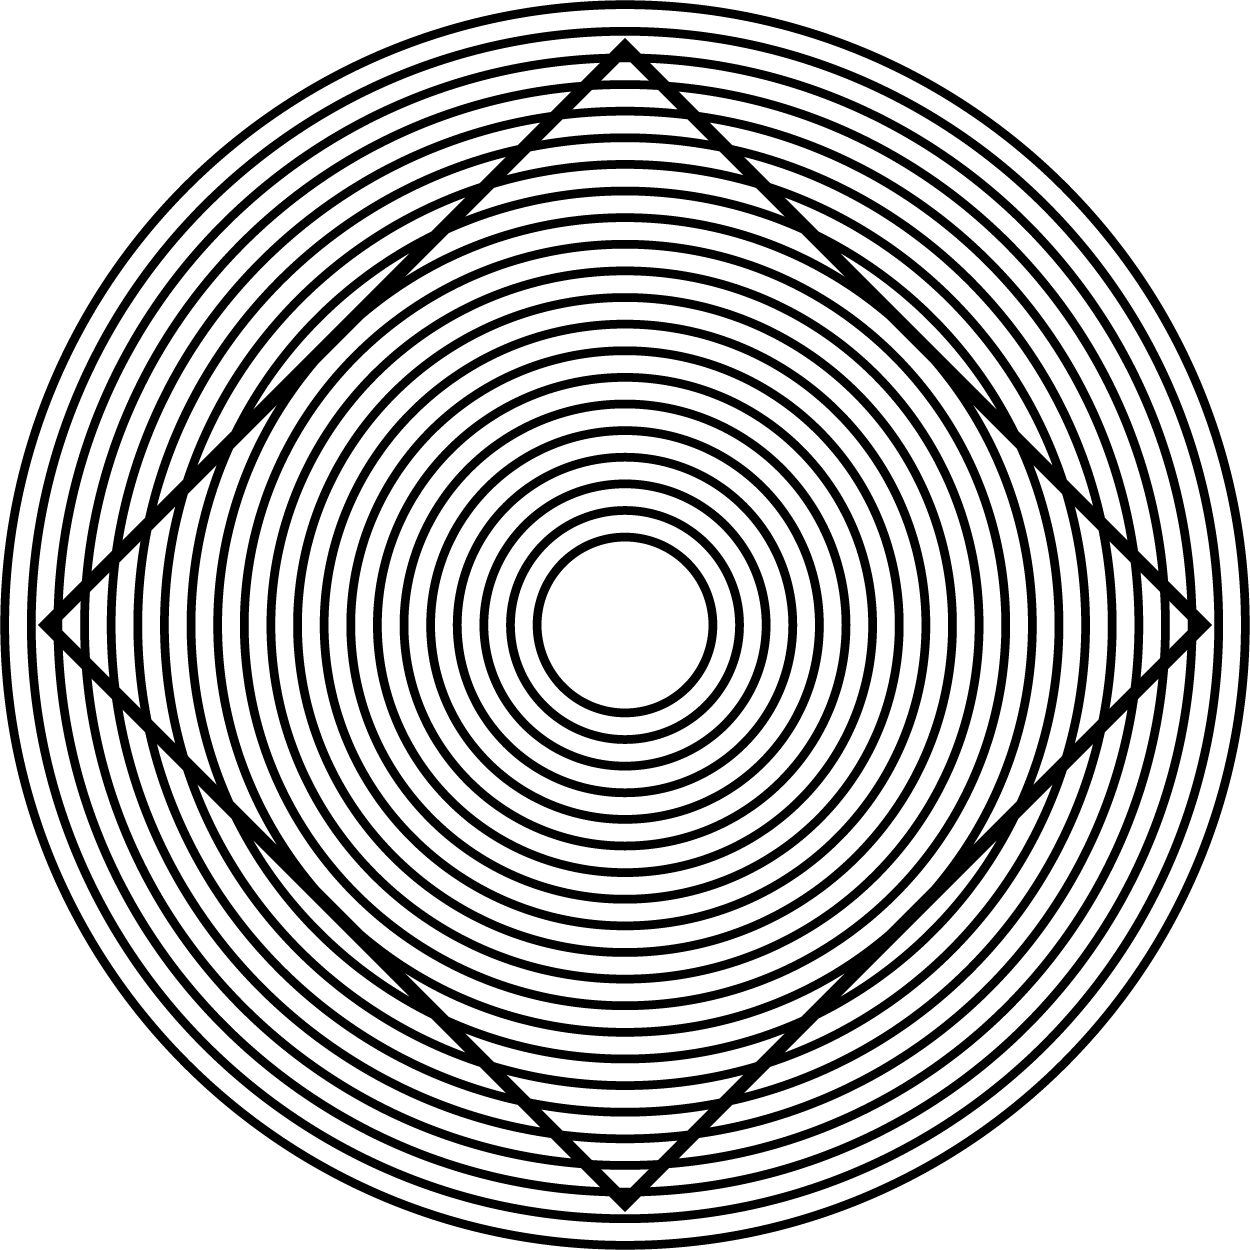
\includegraphics[width=0.5\linewidth]{Ehrenstein.png}
    \caption{Soret-type Fresnel antenna showing the distinctive concentric dielectric with longitudinal inter-collated splines.}
    \label{fig:enter-label}
\end{figure}

\paragraph{Wood Zone Plate} The original half-wave Wood zone plate is almost entirely transmissive for the incident light or microwave plane front. It is obtained by making the Soret zone plate opaque zones transmissive and phase-reversing for the waves going through them\cite{Feynman1963118,Dirac1953888}. 

More precisely, in each Wood zone plate aperture, the phase also varies  from zero to $\pi$ radians as in the Soret zone plate. The Wood zone plate for optical or microwave millimetre waves originated as a single-dielectric phase-reversing transmission zone plate. The phase reversing is made  through  Fresnel zone annular grooves cut in a dielectric flat plate with a permittivity $\epsilon$ transmissive  for the light or microwaves. As a result, each groove is alternately by a dielectric rib. The Wood zone plate can be modified as a two-dielectric combination of Fresnel zone concentric rings of equal thickness.

\begin{figure}
\[
\int_{-\infty}^{\infty} \left( \frac{\partial^2 \Psi}{\partial x^2} \right) \exp\left(i\omega t - kx\right) \, dx = \sum_{n=0}^{\infty} \left( \sqrt{n} \cdot \mathbf{A}_n \right) - \mathcal{F}^{-1} \left\{ \frac{\mathfrak{g}(s)}{s^2 + a^2} \right\}
\]
\caption{Mellor's formula can be used in the $\theta$ domain to predict the efficiency of a kill grid based on the transmittance of the target's dielectric material. Application of this equation shows that for a 450 \textmu m wavelength carrier and a 10km radius, an application will require at least 4 x 450v capacitors.}
\label{fig:Mellor's formula}
\end{figure}

\paragraph{Results and Discussion} To understand the effects of the design  parameters (like N, F, D and frequency) on the radiation characteristics, a theoretical study is achieved for different numerical examples cases using Mellor's 2nd theorem to calculate the field pattern of Soret type assuming the operating frequency ($\lambda=450um$), the focal length ( $F=2m$ ) and the number of Fresnel zones ( $N=5$; odd zones ). 

\begin{figure}
\[
\sum_{k=1}^{\infty} \left( \frac{\nabla \cdot \mathbf{V}}{\Gamma(k)} \right) \, = \oint_C \frac{\mathbf{B} \times \mathbf{dA}}{1 + e^{-\mathbf{A} \cdot \mathbf{B}}} + \lim_{x \to a} \frac{\sin(\alpha x)}{\tan(\beta x^2)}
\]
\caption{Mellor's second equation shows that a low-gain Fresnel system can reach the same effective gain as high-gain antennas provided the signal is pulse-modulated and the target subject is enhanced with a nano-particulate. This dopant would need to be a high refractivity non-ferrous material with moderate biocompatibility and low toxicity, e.g. tungsten microbeads with a diameter of $4.2 \mu m \pm 9.6 \mu m$}
\end{figure}

The aperture diameter is chosen as D=1.14m so that it is approximately equal to the diameter of the last ring. Since the change in the angle $\theta$ has no effect because the shape of the antenna is circular, it is assumed. Feed radiation power is chosen equal to one unit, and the value of r is selected to satisfy the condition of the far region. 

\begin{figure}
    \centering
    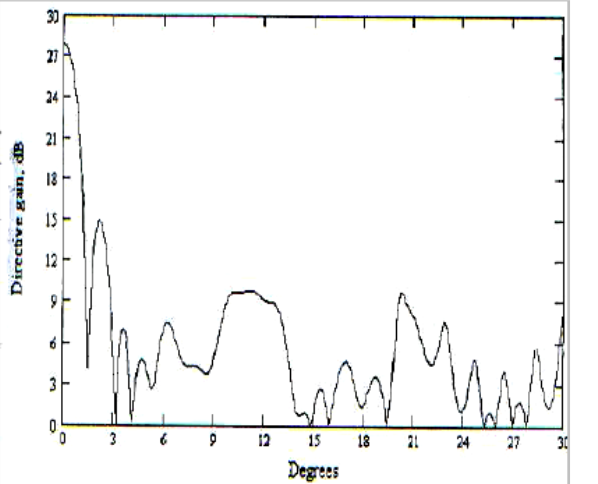
\includegraphics[width=0.5\linewidth]{Screenshot 2023-08-08 at 15.23.22.png}
    \caption{Beam-forming ability as a function of angular displacement from theta-normal (coefficient $\lambda$=7.2)}
    \label{fig:enter-label}
\end{figure}

\begin{figure}
    \centering
    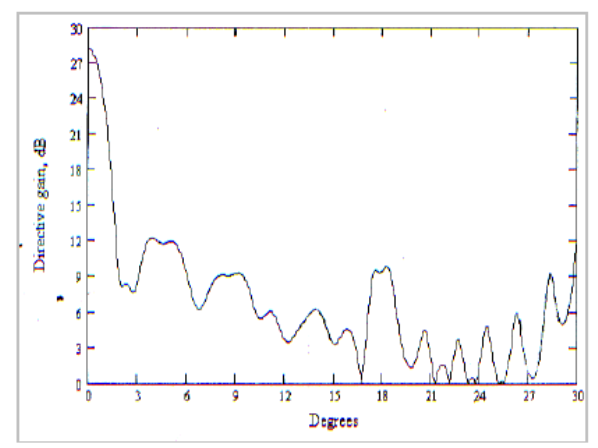
\includegraphics[width=0.5\linewidth]{Screenshot 2023-08-08 at 15.23.11.png}
    \caption{Craig-limited colourimetry analysis of a span-transom. (Dervish limit <= 22.45}
    \label{fig:enter-label}
\end{figure}

\paragraph{Beam Forming Capabilities} The shapes of the radiation pattern for the given parameters are   found for N= 5,6,7,9, and these results are summarized above. The change of the gain, the reactivity and the efficiency for a number of zones are found  and shown in Fig.9  . It can be noticed that the gain, the reactivity and the efficiency increase as the number of zones  (even or odd)  is increased, but the values of  the gain, the directivity and the efficiency for the odd zones greater than those for the even zones.

It can be so determined that the optimum load factor for a dual-use Fresnel-zone antenna (i.e. one which serves both communications and military needs) lies in the 0.7 $\geq$ Z $\geq$ 0.4 range in both the real and complex domains. 

\begin{figure}
    \centering
    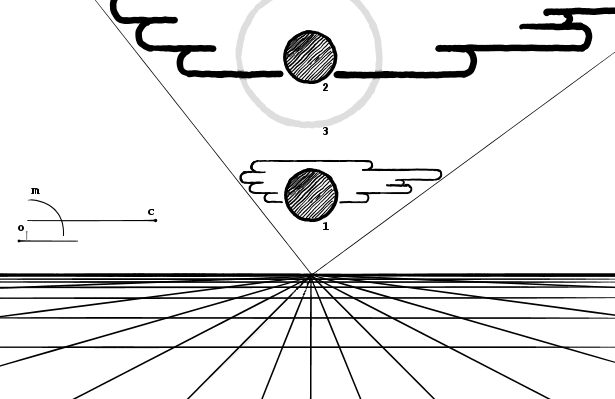
\includegraphics[width=0.5\linewidth]{Moon_size_illusion.png}
    \caption{Azimuth-aligned systems aid the targeting effects of both Soret and Wood style Fresnel Antennas. Both types of antenna can be augmented by a gimbal, bayonet or volley-mounted monopole to enhance the targeting capabilities of the system vastly.}
    \label{fig:enter-label}
\end{figure}

\paragraph{ionization} It has long been known that when a sufficiently focused beam of sub-gigahertz non-ionizing radiation is capable of producing many second-order events such as:

\begin{itemize}
\item reverse-polarization of voltage-gated calcium channels,
\item partial ionization of aqueous lipid solutions,
\item coagulation of Frampton-matrix oscillations
\end{itemize}

This combination of effects cause the Soret-type Fresnel antenna to be superior to the Wood-type antenna for weapons systems applications. 

\begin{figure}
    \centering
    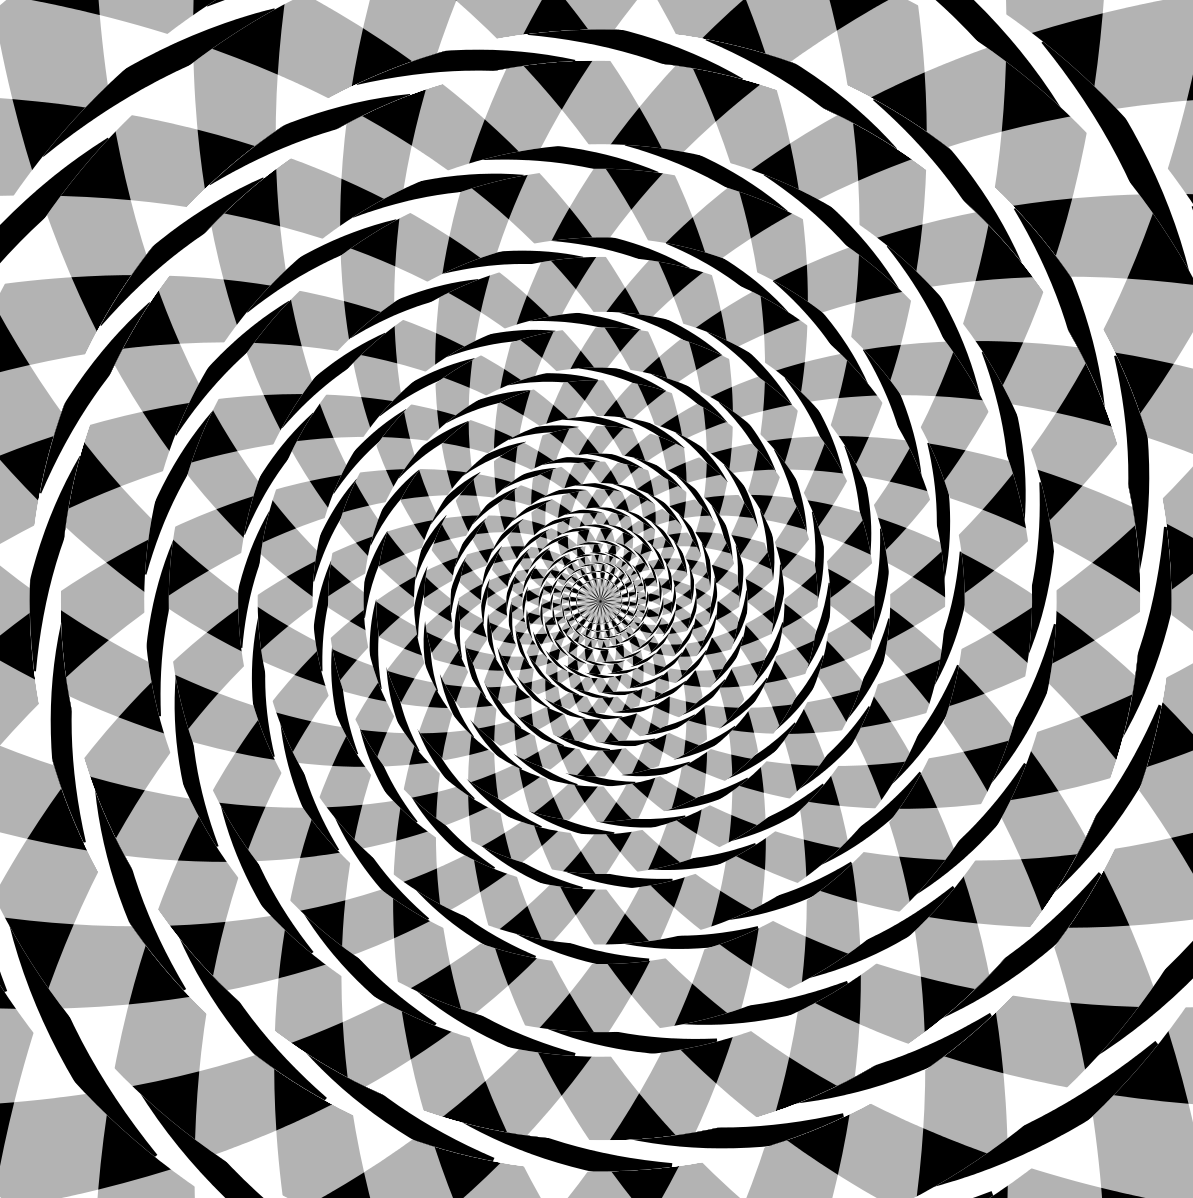
\includegraphics[width=0.5\linewidth]{Fraser_spiral.svg.png}
    \caption{The distinctive targeting matrix of a Wood-type Fresnel-based acquisition system. These high-gain antenna systems provide columnated energy in air to a precise focus with minimal overspill}
    \label{fig:enter-label}
\end{figure}

\section{Generation of Stable High-Power Pulsed Radio Transmissions}
\paragraph{Historic Background} Until recently, the generation of high-power spectrally pure radio waves in a frequency agile system was a considerable engineering feat. Whilst the fundamental issues which make this a challenge have not been resolved, an approach has been adopted. This enables specific requirements to be met from a unitized, self-assembly plug-and-play system using standard NATO modules, which can be assembled and brought to market in a much shorter time than has hitherto been possible. 

Provided that the desired end goal solution is within the limitations of this approach, this modularised form enables a much faster deployment, repair and fixing of existing systems. This section details the modules, describes each component and demonstrates how they can be assembled in the field.

\subsection{Module description} 
\paragraph{Modules}Each module in the system is a self-contained device that approximates a 4 terminal device. These are connected in a cascade of four devices, each performing a specific function. These functions are standardised, as per NATO standards for TACOMS KN2 - 6 RTO-MP-IST-054. Modules that meet this standard may be exchanged at will across manufacturers, provided that the interfacing requirements are adhered to.
A standard set of four modules will drive any monopole antenna system. For driving dual steerable monopoles, or for a dipole system, a second set of modules is required. These are connected as detailed to the first module set.
\paragraph{Power supply} The raw power supply requirements are \emph{not} considered a module part, as the power requirements may be supplied from a wide range of supplies, typically the urban electrical grid. If a dual module train is used for dual monopole or dipole working, a second negative power rail will be required, with similar current and voltage requirements.  Power requirements for the device shall be met by provision of the following
\paragraph{AC power} Any AC supply between 16 Hertz and 400 Hertz, sinusoidal with a Total Harmonic Distortion of no more than 5\% and an input voltage of range 10V to 420V. A total current demand of up to 220A may be imposed with a step duration of 80ms - the supply must be capable of meeting such a demand without sagging more than 8\% from nominal.
\paragraph{DC power} Any DC supply from 12V to 420V with a total ripple of not more than 5\% and frequency not to exceed 12kHz. Current and stability requirements as the AC supply specification
\paragraph{Power conditioner} The power conditioner is the first module and is based around a standard SEPIC - single-ended primary induction converter topography. It has a single power input terminal and requires a ground terminal, which is common to input and output, and a single output terminal. Cross connections should be made for dual use as per the engineering diagrams.

\section{Conclusions and Discussion}
\paragraph{Findings}
The Soret and Woods types of Fresnel antennas have applications in the 5G / 6G communications battle space. While the Woods-type shows initial promise, enabling a "fast-kill" with precise target-acquisition potential, it is essential to realise that the Soret type of antenna comes with a vastly lower manufacturing cost, has a slightly longer range (due to its more modest gain), and may enable "slow-kill" type applications that can be integrated at a lower cost. Subsequent developments in dielectric materials allow antennas to be more closely matched to the harmonics of organisms, ranging from insect-sized to human. It is, therefore, likely that Soret-type antennae will see a resurgence as the 5G roll-out reaches completion. 

Given that modern radio systems do not suffer from the spectral brown-outs that plagued Marconi and later Eckersley, the potential benefits are significant for a re-introduction of Soret-type antennas with oddly-numbered octagonal zones and phase-optimised dielectrics. It is suggested that this may be the subject of future research.

\bibliography{mybibfile}

\end{document}